\documentclass[finalspec]{sbmlpkgspec}
%%\documentclass[draftspec]{sbmlpkgspec}
\usepackage{microtype}
\usepackage{color}

\usepackage{todonotes}
\usepackage{subfigure}
\usepackage{longtable}
\usepackage[color]{changebar}
\usepackage{xcolor}
\usepackage{soul}

\usepackage[final]{pdfpages}

% putting versions on changebars
\newcommand{\version}[2]{\marginpar{\hspace*{34pt}\raisebox{-3.0ex}{\color{#1}\small #2}}}

%% ============================================================================
%% Description:  Documentation for sbmlpkgspec.cls
%% First author: Michael Hucka <mhucka@caltech.edu>
%% Organization: California Institute of Technology
%% Date created: September 2011
%% https://sbml.svn.sourceforge.net/svnroot/sbml/trunk/project/tex/sbmlpkgspec
%%
%% Copyright (C) 2011-2012 California Institute of Technology, Pasadena, CA.
%%
%% SBMLPkgSpec is free software; you can redistribute it and/or modify it
%% under the terms of the GNU Lesser General Public License as published by
%% the Free Software Foundation.  A copy of the license agreement is provided
%% in the file named "LICENSE.txt" included with this software distribution.
%% ============================================================================

% Macros just for this document:

\newcommand{\sbmlpkg}{\texorpdfstring{%
    \textls[-25]{\textsc{SBMLPkgSpec}}}{%
    \textsc{SBMLPkgSpec}}\xspace}
\newcommand{\sbmlpkghead}{\texorpdfstring{%
    \textls[-50]{\textsc{SBMLPkgSpec}}}{%
    \textsc{SBMLPkgSpec}}\xspace}
\newcommand{\sbmlpkgfile}{\literalFont{sbmlpkgspec.cls}\xspace}
\newcommand{\latex}{\LaTeX{}\xspace}
\newcommand{\tex}{\TeX{}\xspace}
\newcommand{\distURL}{http://sourceforge.net/projects/sbml/files/specifications/tex}
\newcommand{\srcURL}{https://sbml.svn.sourceforge.net/svnroot/sbml/trunk/project/tex/sbmlpkgspec}
\newcommand{\webURL}{http://sbml.org/Documents/Specifications/The_SBMLPkgSpec_LaTeX_class}
\newcommand{\cmd}[1]{\literalFont{\textbackslash #1}}

% Custom latex listing style, for use with the listings package.  The default
% highlights far too many things, IMHO.  This keeps it simple and only adjusts
% the appearance of comments within listings.

\lstdefinelanguage{mylatex}{%
  morekeywords={},%
  sensitive,%
  alsoother={0123456789$_},%$
  morecomment=[l]\%%
}[keywords,tex,comments]

\lstdefinestyle{latex}{language=mylatex}


%Listing style for SBOL RDF/XML serialization examples
\usepackage{listings}
\usepackage{color}
\usepackage{xcolor} 
\definecolor{dkgreen}{rgb}{0,0.6,0}
\definecolor{gray}{rgb}{0.5,0.5,0.5}
\definecolor{light-gray}{gray}{0.97}
\lstdefinelanguage{sbol}
    {morekeywords={xmlns:sbol,rdf:about,sbol:displayId,sbol:persistentIdentity,sbol:version,sbol:timeStamp,sbol:name,sbol:description,sbol:member,sbol:Collection,sbol:type, sbol:role, sbol:ComponentDefinition, sbol:MapsTo, sbol:sequence,sbol:wasDerivedFrom,sbol:Component,sbol:subComponent,sbol:SequenceAnnotation,sbol:component,sbol:location, sbol:sequenceAnnotation, sbol:Range, sbol:start, sbol:end, sbol:orientation,sbol:SequenceConstraint, sbol:restriction, sbol:subject, sbol:object,sbol:Sequence, sbol:elements, sbol:encoding,sbol:Model, sbol:source, sbol:language, sbol:framework,sbol:FunctionalComponent, sbol:Module, sbol:Interaction, sbol:interaction, sbol:module, sbol:model,sbol:Model,sbol:definition, sbol:access, sbol:direction, sbol:mapsTo, sbol:refinement, sbol:local, sbol:remote, sbol:participation, sbol:Participation, sbol:participant,sbol:sequenceConstraint,sbol:at,sbol:Cut,sbol:functionalComponent,sbol:ModuleDefinition,prov:wasDerivedFrom,dcterms:title,dcterms:description},
     basicstyle=\fontsize{7}{9}\selectfont\ttfamily,
     backgroundcolor=\color{light-gray},
     keywordstyle=\color{blue},
     commentstyle=\color{gray},
     stringstyle=\color{dkgreen},
     tabsize=2,
     showspaces=false,
     showstringspaces=false,
     breaklines=true,                           % wrap text
     sensitive=true,                            % keywords are case sensitive
     %morecomment=[l][commentstyle]{\#},         % comment format
     morestring=[b]",                           % string format
     escapeinside={[}{]},
     alsoletter=:
     %breakatwhitespace=true, 
     %literate={\-}{}{0\discretionary{a}{\\}{}}
}

%Command to format the listings containing SBOL RDF/XML serialization examples
\newcommand{\lstsetsbol}{
 \lstset{language=sbol,
        tabsize=2
 }
}

%Commands to format SBOL terms in the document
\newcommand{\sbolheading}[1]{\texttt{#1}}
\newcommand{\sbol}[1]{\texttt{#1}} % no hyperrefs, because they're in a different document
%\newcommand{\sbol}[1]{\texttt{\hyperref[sec:#1]{#1}}}
%\newcommand{\sbolmult}[2]{\texttt{\hyperref[sec:#1]{#2}}}
\newcommand{\refObj}[1]{$\langle$#1$\rangle$}

%Command to format external terms in the document
\newcommand{\external}[1]{\texttt{#1}}

% Commands to track certain TODO nodes in document:
\newcommand{\todoresolved}[1]{\todo[color=blue, inline]{{\bf Resolved:} {\it #1}}}
\newcommand{\actionitem}[1]{\todo[color=green, inline]{#1}}
\newcommand{\tododeferred}[1]{\todo[color=cyan, inline]{#1}}
\newcommand{\todoquery}[1]{\todo[color=yellow, inline]{DECISION NEEDED: #1}}
\newcommand{\todocritical}[1]{\todo[color=red, inline]{CRITICAL ISSUE: #1}}

% -----------------------------------------------------------------------------
% Start of document
% -----------------------------------------------------------------------------
%Commands to highlight SBOL versions
\newcommand{\twoonezero}[1]{%
\cbcolor{red}
\cbstart%
{\color{red}%
\version{red}{2.1.0}%
#1
}
\cbend
}

% version that avoids undesirable page break in glyph collections
\newcommand{\twoonezeronopage}[1]{%
\cbcolor{red}
\cbstart%
{\color{red}%
#1
}
\cbend
}

\newcommand{\twotwozero}[1]{%
\cbcolor{magenta}
\cbstart%
{\color{magenta}%
\version{magenta}{2.2.0}%
#1
}
\cbend
}

% version that avoids undesirable page break in glyph collections
\newcommand{\twotwozeronopage}[1]{%
\cbcolor{magenta}
\cbstart%
{\color{red}%
#1
}
\cbend
}


% -----------------------------------------------------------------------------
% Start of document
% -----------------------------------------------------------------------------

\begin{document}

\packageTitle{\latex Class for SBML Package Specifications}
\packageVersion{Version 2.2}
\packageVersionDate{March, 2020}

% BBF RFC \rfcnum{}: 
\title{Synthetic Biology Open \\Language Visual (SBOL Visual) Version~2.2}


\author{{\bf Editors:}\hfil\\
\begin{tabular}{l>{\hspace*{15pt}}r}
Hasan Baig & \emph{Habib University}\\
Pedro Fontanarrosa & \emph{University of Utah}\\
Vishwesh Kulkarni & \emph{University of Warwick}\\
James McLaughlin & \emph{Newcastle University, UK}\\
Prasant Vaidyanathan & \emph{Microsoft Research, UK}\\
\end{tabular}\\
{\bf Chair:}\hfil\\
\begin{tabular}{l>{\hspace*{15pt}}r}
Chris Myers & \emph{University of Utah, USA}\\
\end{tabular}\\
\href{mailto:editors@sbolstandard.org}{\sffamily editors@sbolstandard.org}\\
{\bf Additional authors, by last name:}\\
\begin{small}
\begin{tabular}{l>{\hspace*{15pt}}r}
Bryan Bartley & \emph{Raytheon BBN Technologies, USA}\\
Jacob Beal & \emph{Raytheon BBN Technologies, USA}\\
Swapnil Bhatia & \emph{Boston University, USA}\\
Shyam Bhakta & \emph{Rice University, USA}\\
Michael Bissell & \emph{Shipyard Toolchains LLC, USA}\\
Kevin Clancy & \emph{Thermo Fisher Scientific, USA}\\
Robert Sidney Cox & \emph{Kobe University, Japan}\\
Angel Goni Moreno & \emph{Newcastle University}\\
Thomas Gorochowski & \emph{University of Bristol, UK}\\
Raik Grunberg &\emph{KAUST, Saudi Arabia}\\
Augustin Luna & \emph{Harvard Medical School, USA}\\
Curtis Madsen & \emph{Sandia National Laboratories, USA}\\
Goksel Misirli & \emph{Keele University, UK}\\
Tramy Nguyen & \emph{University of Utah, USA}\\
Nicolas Le Novere & \emph{Babraham Institute, UK}\\
Zachary Palchick & \emph{Zymergen, USA}\\
Matthew Pocock & \emph{Turing Ate My Hamster, Ltd., UK}\\
Nicholas Roehner & \emph{Raytheon BBN Technologies, USA}\\
Herbert Sauro & \emph{University of Washington, USA}\\
James Scott-Brown & \emph{Imperial College, UK}\\
John T. Sexton & \emph{Rice University, USA}\\
Guy-Bart Stan & \emph{Imperial College, UK}\\
Jeffrey J. Tabor & \emph{Rice University, USA}\\
Marta Vazquez Vilar & \emph{Universitat Politecnica de Valencia, Spain}\\
Chris Voigt & \emph{MIT, USA}\\
Anil Wipat & \emph{Newcastle University, UK}\\
David Zong & \emph{Rice University, USA}\\
Zach Zundel & \emph{University of Utah, USA}\\
%\bf{and also any others} & \bf{who believe they should be authors} \\
\end{tabular}
\end{small}
}

% Non-contributing editors who do not qualify for authorship after their term expires:
%Umesh P & \emph{Kerala Technological University, India}\\


\maketitlepage
%\tododeferred{Confirm date, authors, turn off draft mode}

\maketableofcontents


% -----------------------------------------------------------------------------
\section{Purpose}
% -----------------------------------------------------------------------------

People who engineer biological organisms often find it useful to draw diagrams in order to
communicate both the structure of the nucleic acid sequences that they are engineering
and the functional relationships between sequence features and other molecular species.
%
Some typical practices and conventions have begun to emerge for such
diagrams.  SBOL Visual aims to organize and systematize such
conventions in order to produce a coherent language for expressing
the structure and function 
of genetic designs. 
%
At the same time, we aim to make this language simple and easy to use,
allowing a high degree of flexibility and freedom in how such diagrams are organized, presented, and
styled---in particular, it should be readily possible to create
diagrams either by hand or using a wide variety of software programs.
%
Finally, means are provided for extending the language with new and
custom diagram elements, and for adoption of useful new elements into
the language.

\subsection{Relation to Data Models}

In order to ground SBOL Visual with precise definitions, we reference its visual elements to data models with well-defined semantics.
In particular, glyphs in SBOL Visual are defined in terms of their relation to the SBOL 2 data model (as defined in BBF RFC 112) and terms in the Sequence Ontology~\citep{SequenceOntology} and
the Systems Biology Ontology~\citep{SBO}.

SBOL Visual is not intended to represent designs at the same level of detail as these data models.
Effective visual diagrams are necessarily more abstract, focusing only on those aspects of a system that are the subject of the communication.
Nevertheless, we take as a principle that it should be possible to transform any SBOL Visual diagram into an equivalent (if highly abstract) SBOL 2 data representation.
Likewise, we require that SBOL Visual should be able to represent all of the significant structural or functional relationships in any GenBank or SBOL data representation.


\nopagesection{Relation to other Standards}

SBOL Visual 3.0 replaces SBOL Visual 2.3.
%
%Substantive differences between SBOL Visual 2.3 and prior versions of SBOL Visual 2 are marked with change bars identifying the version in which the new material was introduced.

SBOL Visual 2.3 also implicitly supersedes the previously replaced SBOL Visual 2.2 and 2.1, as well as BBF RFC 115 (SBOL Visual 2.0), BBF RFC 93 (SBOL Visual 1.1) and BBF RFC 16 (SBOL Visual 1.0).

Every glyph in SBOL Visual 3.0 corresponds to an element of the SBOL 3.0 data model.
SBOL Visual 3.0 also defines many terms by reference to SBOL 3.0, 
or by reference to the Sequence Ontology~\citep{SequenceOntology}
or the Systems Biology Ontology~\citep{SBO}.

SBOL Visual is intended to be compatible with the Systems Biology Graphical Notation Activity Flow Language (SBGN AF)~\citep{sbgn}, 
and species and interaction glyphs have been imported from that language (see: \ref{apdx:sym:species} and \ref{apdx:sym:interaction}).
Some aspects are also imported from the Systems Biology Graphical Notation Process Description Language (SBGN PD).


% -----------------------------------------------------------------------------
\section{SBOL Specification Vocabulary}
% -----------------------------------------------------------------------------

\subsection{Term Conventions}

% Note: yes, it's really RFC 0
This document indicates requirement levels using the controlled vocabulary specified in IETF RFC 2119 and reiterated in BBF RFC 0.
In particular, the key words "MUST", "MUST NOT", "REQUIRED", "SHALL", "SHALL NOT", "SHOULD", "SHOULD NOT", "RECOMMENDED", "MAY", and "OPTIONAL" in this document are to be interpreted as described in RFC 2119:

\begin{itemize}
\item The words "MUST", "REQUIRED", or "SHALL" mean that the item is an absolute requirement of the specification.
\item The phrases "MUST NOT" or "SHALL NOT" mean that the item is an absolute prohibition of the specification.
\item The word "SHOULD" or the adjective "RECOMMENDED" mean that there might exist valid reasons in particular circumstances to ignore a particular item, but the full implications need to be understood and carefully weighed before choosing a different course.
\item The phrases "SHOULD NOT" or "NOT RECOMMENDED" mean that there might exist valid reasons in particular circumstances when the particular behavior is acceptable or even useful, but the full implications need to be understood and the case carefully weighed before implementing any behavior described with this label.
\item The word "MAY" or the adjective "OPTIONAL" mean that an item is truly optional.
\end{itemize}

\subsection{SBOL Class Names}

\todo[inline]{Change to use SBOL 3.0 class names}

The definition of SBOL Visual references several SBOL classes, which are defined as listed here.  For full definitions and explanations, see BBF RFC 112, describing the SBOL 2.1 data model.

\begin{description}

%\item \emph{\sbol{Collection}}:
%Represents a user-defined container for organizing a group of SBOL objects.

\item \emph{\sbol{ComponentDefinition}}: Describes the structure of designed entities, such as DNA, RNA, and proteins, as well as other entities they interact with, such as small molecules or environmental properties.

\begin{itemize}
\item \emph{\sbol{Component}}:
Pointer class. Incorporates a child \sbol{ComponentDefinition} \textit{by reference} into exactly one parent \sbol{ComponentDefinition}. Represents a specific occurrence or instance of an entity within the design of a more complex entity. Because the same definition might appear in  multiple designs or multiple times in a single design, a single \sbol{ComponentDefinition} can have zero or more parent \sbol{ComponentDefinition}s, and each such parent-child link requires its own, distinct \sbol{Component}.

\item \emph{\sbol{Location}}:
Specifies the base coordinates and orientation of a genetic feature on a DNA or RNA molecule or a residue or site on another sequential macromolecule such as a protein.

\item \emph{\sbol{SequenceAnnotation}}:
Describes the \sbol{Location} of a notable sub-sequence found within the \sbol{Sequence} of a \sbol{ComponentDefinition}. Can also link to and effectively position a child \sbol{Component}.

\item \emph{\sbol{SequenceConstraint}}:
Describes the relative spatial position and orientation of two \sbol{Component} objects that are contained within the same \sbol{ComponentDefinition}.
\end{itemize}

%\item \emph{\sbol{GenericTopLevel}}:
%Represents a data container that can contain custom data added by user applications.

%\item \emph{\sbol{Model}}:
%Links to quantitative or qualitative computational models that might be used to predict the functional behavior of a biological design.

\item \emph{\sbol{ModuleDefinition}}:
Describes a ``system'' design as a collection of biological components and their functional relationships.

\begin{itemize}
\item \emph{\sbol{FunctionalComponent}}:
Pointer class. Incorporates a child \sbol{ComponentDefinition} \textit{by reference} into exactly one parent \sbol{ModuleDefinition}. Represents a specific occurrence or instance of an entity within the design of a system. Because the same definition might appear in multiple designs or multiple times in a single design, a single \sbol{ComponentDefinition} can have zero or more parent \sbol{ModuleDefinition}s, and each such parent-child link requires its own, distinct \sbol{FunctionalComponent}.

\item \emph{\sbol{Interaction}}:
Describes a functional relationship between biological entities, such as regulatory activation or repression, or a biological process such as transcription or translation.

\twoonezero{
\item \emph{\sbol{MapsTo}}:
When a design (\sbol{ComponentDefinition} or \sbol{ModuleDefinition}) includes another design as a sub-design, the parent design might need to refer to a \sbol{ComponentInstance} (either a \sbol{Component} or \sbol{FunctionalComponent}) in the sub-design.
In this case, a \sbol{MapsTo} needs to be added to the instance for the sub-design, and this \sbol{MapsTo} needs to link between the \sbol{ComponentInstance} in the sub-design and a \sbol{ComponentInstance} in the parent design.

\item \emph{\sbol{Module}}:
Pointer class. Incorporates a child \sbol{ModuleDefinition} \textit{by reference} into exactly one parent \sbol{ModuleDefinition}. Represents a specific occurrence or instance of a subsystem within the design of a larger system. Because the same definition in multiple designs or multiple times in a single design, a single \sbol{ModuleDefinition} can have zero or more parent \sbol{ModuleDefinition}s, and each such parent-child link requires its own, distinct \sbol{Module}.
}

\item \emph{\sbol{Participation}}:
Describes the role that a \sbol{FunctionalComponent} plays in an \sbol{Interaction}.
For example, a transcription factor might participate in an \sbol{Interaction} as a repressor or as an activator.

\end{itemize}

%\item \emph{\sbol{Sequence}}:
%Generally represents a contiguous series of monomers in a macromolecular polymer such as DNA, RNA, or protein. A \sbol{Sequence} can also encode the atoms and bonds of a molecule with non-linear structure (see \ref{sec:Sequence}).

\end{description}

% -----------------------------------------------------------------------------
\section{SBOL Glyphs}\label{sec:glyphs}
% -----------------------------------------------------------------------------

A glyph is a visual symbol used to represent an element in an SBOL Visual diagram.
All of the currently defined glyphs are collected in \ref{apdx:symbols}.
%
This section explains how glyphs are specified and how to add new glyphs.

Each SBOL glyph is defined by association with ontology terms, and can be used to represent any diagram element that is well-described by that term.
Currently there are four classes of glyphs, each associated with an ontology and a class in the SBOL 3 data model:
\begin{itemize}
\item {\bf Sequence Feature Glyphs} describe features of nucleic acid sequences. 
They are associated with Sequence Ontology terms.
For the SBOL 3 data model, this is formally defined as any \sbol{Feature} with a compatible term within its associated \sbol{roles},
 i.e., one that is equal to or a child of at least one term associated with the glyph.

\item {\bf Molecular Species Glyphs} represent any class of molecule whose detailed structure is not being shown using sequence feature glyphs. 
They are associated with Systems Biology Ontology terms. 
 For the SBOL 3 data model, this is formally defined as any \sbol{Feature} with a compatible term within its associated \sbol{types},
 i.e., one that is equal to or a child of at least one term associated with the glyph.

\item {\bf Interaction Glyphs} are ``arrows'' indicating functional relationships between sequence features, molecular species, and/or other relationships. 
They are associated with Systems Biology Ontology terms.
For the SBOL 3 data model, this is formally defined as any \sbol{Interaction} with a compatible term within its \sbol{types},
 i.e., one that is equal to or a child of at least one term associated with the glyph, 
 and with a compatible \sbol{Participation} at the head and tail of the arrow.

\item {\bf Interaction Node Glyphs} are placed at the junctions of edges to represent biochemical processes.
They are associated with Systems Biology Ontology terms.
For the SBOL 3 data model, this is formally defined as any \sbol{Interaction} with a compatible term within its \sbol{types},
 i.e., one that is equal to or a child of at least one term associated with the glyph, 
 and with a compatible \sbol{Participation} on the incoming and outgoing edges of the glyph
 \end{itemize}
 
More than one glyph may share the same definition: in this case, these glyphs form a family of variants, of which precisely one MUST be designated as the RECOMMENDED glyph, which is to be used unless there are strong reasons to prefer an alternative variant.

It will also frequently be the case that a diagram element could be represented by more than one glyph (e.g., a glyph for a specific term and a glyph for a more general term).
In such cases, it is RECOMMENDED that the most specific applicable glyph be used.
However, if upward branching in the relevant ontology means two applicable glyphs do not have an ordered parent/child relation, then either MAY be used.

For example, a protein coding sequence (CDS) is a sequence feature that may be represented either using the CDS glyph (Sequence Ontology term SO:0000316) or the Unspecified glyph (Sequence Ontology term SO:0000001).  
Since SO:0000316 is contained by SO:0000001, the preferred glyph is CDS, rather than Unspecified.
Likewise, a CDS may be represented by either a pentagonal glyph or an arrow glyph, but the pentagon is the RECOMMENDED variant, and so it is likewise preferred.  
\ref{f:glyphalternatives} illustrates this example.

\begin{figure}[h!]
\centering
\includegraphics[scale=0.6]{figures/glyphalternatives.pdf}
\caption{A biological design element such as a protein coding sequence (CDS) is best represented by the most specific RECOMMENDED glyph (middle), but can be represented by a less specific glyph such as Unspecified (left) or an approved alternative glyph (right).}
\label{f:glyphalternatives}
\end{figure}

Finally, note that the mapping from data model to glyph is not one-to-one: many SBOL 3 data model constructs can, at least in theory, be represented visually in multiple different ways. 
For example, a DNA construct carrying a heterologous gene could be represented by the molecular species glyph for a double-stranded nucleic acid, the sequence feature glyph for an engineered construct, or a series of sequence feature glyphs showing the internal structure of the gene.
This ambiguity is deliberate allowing diagrams to select an appropriate level of detail for the information that a diagram is intended to convey.

\subsection{Requirements for Glyphs}

\todo[inline]{Do we need to add to these for parametric?}

A number of requirements are placed on all SBOL Visual glyphs in order to
ensure both the clarity of diagrams and the ease with which they can
be constructed:
\begin{enumerate}
\item A glyph SHOULD have its meaning defined by associating the glyph with at least one ontology definition.
	Definitions are RECOMMENDED to be from the Sequence Ontology for sequence feature glyphs, from the Systems Biology Ontology for molecular species glyphs, and from the Systems Biology Ontology for interaction glyphs.  
	If no applicable terms are available in the preferred ontology, proposal of a new glyph SHOULD be accompanied by a request to the ontology maintainers to add a term for the undefined entity.  
\item A glyph SHOULD be relatively easy to sketch by hand (e.g., no high-complexity images or precise angles required).
\item A glyph specification MUST indicate which portions of the glyph are the ``interior'' for purposes of color fill.
\item A glyph specification SHOULD show the glyph in its preferred relative scale with respect to other glyphs.
\item A glyph SHOULD be specified using only solid black lines (leaving color and style to be determined by the user, as noted below).
\item A glyph SHOULD NOT be similar enough to be easily confused with any other glyph when written by hand, or when scaled either vertically, horizontally, or both.
\item A glyph SHOULD NOT include text (note that associated labels are not part of the glyph).
\end{enumerate}

In addition, some requirements apply only to certain classes of glyphs:
\begin{enumerate}[resume]
\item A sequence feature or molecular species glyph specification MUST include a rectangular bounding box indicating its extent in space.
\item A sequence feature glyph specification MUST include exactly one horizontal rule for its RECOMMENDED vertical alignment with the nucleic acid backbone.
\item A sequence feature glyph SHOULD be asymmetric on the horizontal axis. Vertical asymmetry is also preferred when possible.
\item If a sequence feature glyph can represent components of highly variable size or structural complexity, the glyph SHOULD be able to be scaled horizontally to indicate relative scale.
\end{enumerate}

\ref{f:specexample} shows examples of compliant glyph specification.

\begin{figure}[h!]
\centering
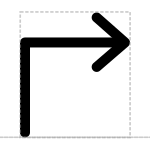
\includegraphics[scale=2.0]{figures/promoter-specification.pdf}

\includegraphics[scale=2.0]{figures/ribosome-entry-site-specification.pdf}
\caption{Examples of glyph specification: this specification for the sequence feature glyphs for Promoter (left) and Ribosome Entry Site (right) include the glyph outline, fill (grey center of Ribosome Entry Site), bounding box (dashed box), and recommended alignment with the nucleic acid backbone (dashed horizontal line), all at a preferred relative scale.}
\label{f:specexample}
\end{figure}

\subsection{Reserved Visual Properties}

SBOL Visual aims to allow as much flexibility and freedom as possible in how diagrams are organized, presented, and styled.
%
To this end, a number of aspects of presentation are generally reserved for the communication of other types of information by the creator of a diagram.
%
When using a glyph in a diagram, the following choices in glyph presentation are thus explicitly intended to be alterable:
\todo[inline]{Do we need to add to these for parametric?}
\begin{enumerate}
\item The lines of a glyph MAY be given any line thickness and style
\item The interior of a glyph MAY be given any fill color, as long as the choice of fill does not interfere with recognizing the glyph.
\item The scale of glyphs are RECOMMENDED to be kept consistent with their specification and throughout a diagram, but can be altered if desired, particularly to convey additional information (e.g., length of a sequence).
\item Minor styling effects MAY be chosen (e.g., shadow, corner styling, other "font-level" customization)
\end{enumerate}
\ref{f:stylevariation} shows some examples of acceptable style variation.

In certain special cases, the style of a glyph may be more constrained, but such cases are expected to be rare and strongly motivated.

\begin{figure}[h!]
\centering
\includegraphics[scale=1.0]{figures/style-variation.pdf}
\caption{Examples of acceptable style variation for a Promoter glyph.}
\label{f:stylevariation}
\end{figure}

\subsection{Extending the Set of Glyphs}\label{sec:extension}
The collection of SBOL Visual glyphs is not expected to provide
complete coverage of all of the types of element that people will
wish to include in genetic diagrams, particularly given the ongoing
evolution of synthetic biology as an engineering discipline.
%
As the need for new diagram elements or new practices of usage emerge,
new glyphs or glyph definitions are expected to be added to SBOL
Visual.
%
In particular, the following three classes of changes are expected to occur regularly,
and the SBOL development community will maintain clear processes for
proposal and adoption of changes of this type:
\begin{itemize}
\item New glyphs, either representing a type of component that
  previously lacked a glyph or enabling a distinction between types of
  components previously represented by the same glyph.
\item Additional glyph variants, accompanied by compelling use cases
  that cannot be adequately addressed by the existing glyph variants.
\item Additional definitions for a glyph, capturing an alternate
  meaning that is useful to humans but existing within a disjoint
  branch of the relevant ontology.
\end{itemize}

In order to support the coherent extension of SBOL Visual, 
whenever a diagram creator uses a glyph not found in \ref{apdx:symbols}, 
the creator SHOULD submit it to be considered for inclusion in an updated version of the standard following the processes for adding new glyphs found on the community website at \url{http://sbolstandard.org}





% % -----------------------------------------------------------------------------
\section{SBOL Visual Diagram Language}
\label{sec:language}
% % -----------------------------------------------------------------------------

An SBOL Visual diagram represents information about the structure of a nucleic acid design and its associated molecular species and interactions.
%
If desired, an SBOL Visual diagram may also be associated with a machine-interpretable model (e.g., in SBOL, GenBank, or SBML format).
In this document we describe the association for the SBOL 2 data model, which provides a formal semantic grounding for all elements of an SBOL Visual diagram, but equivalent associations may be made between diagram elements and other models.
%
In terms of the SBOL 2 data model, the description of a nucleic acid design is formally defined as a representation of a \sbol{ComponentDefinition} with a nucleic acid \sbol{type}, the \sbol{Component} and \sbol{SequenceAnnotation} objects describing the features and sub-structure of the design, and \sbol{SequenceConstraint} information on the relative positions of such elements.
%
The description of interactions between some number of nucleic acid designs and other molecular species is formally defined as a representation of a \sbol{ModuleDefinition}, the \sbol{FunctionalComponent} objects describing the nucleic acid designs and other molecular species, and the \sbol{Interaction} and \sbol{Participation} objects describing their functional relationships.

\begin{figure}[h!]
\centering
\includegraphics[width=6in]{figures/SBOLsyntax.pdf}
\caption{Generic syntax of SBOL Visual 2:  
a diagram for a nucleic acid construct is based around a backbone line, its structure specified by the sequence of attached sequence feature glyphs.  
Strand can optionally be indicated by placing a glyph above or below the backbone.  
Other molecular species are indicated by glyphs not in contact with any backbone.
Interactions are directed edges connecting sequence feature or molecular species glyphs.
Any of these objects may have an associated label showing its name, and the diagram may further include any form of other annotations, including other types of text.}
\label{f:syntax}
\end{figure}

\begin{figure}[h!]
\centering
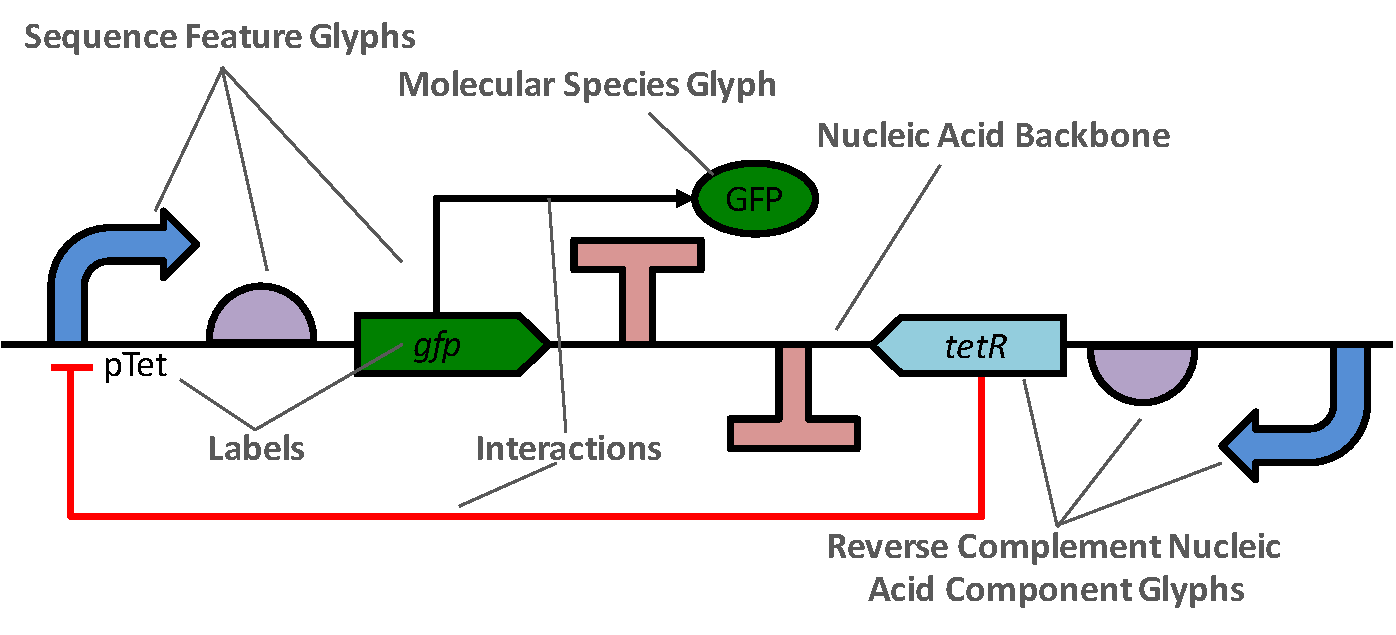
\includegraphics[width=6in]{figures/SBOLgeneral.pdf}
\caption{Example illustrating the elements of an SBOL Visual 2 diagram, with nucleic acid sequence features on the forward and reverse strand of a backbone, other molecular species, and interactions between elements; the grey labels and indicator lines are annotations.}
\label{f:example}
\end{figure}
% inhibition and production relationships

Specifically, an SBOL Visual diagram consists of the classes of objects illustrated in \ref{f:syntax}.
\ref{f:example} shows an example of such a diagram, in a typical usage.
Full details of this specification are provided in the remainder of this section.


\subsection{Nucleic Acid Backbone}
\label{s:lang:backbone}

A diagram for a nucleic acid construct is based around a single or double line, representing the nucleic acid backbone. 
Information about features of the construct can then be represented by attaching nucleic acid glyphs to the backbone, as defined below in \ref{s:lang:nacomponent}.
%
In terms of the SBOL 2 data model, the backbone represents a \sbol{ComponentDefinition} with a nucleic acid \sbol{type} (e.g., DNA, RNA), and the features represent \sbol{Component} and \sbol{SequenceAnnotation} members of the \sbol{ComponentDefinition}.

\begin{enumerate}
\item Lines in some cases indicate strand count. 
	A double-stranded region of the nucleic acid construct MAY use either a single or double line for the backbone.  
	A single-stranded region of the nucleic acid construct MUST use a single line to indicate the backbone.
	When single and double lines are mixed within a single diagram, the single lines always indicate single-stranded regions.
	Examples are provided in~\ref{exa:1a}.
	
	\begin{figure}[h!]
	\centering
	\subfigure[Single- or double-strand backbone]{\includegraphics[scale=0.4]{figures/examples/1a-singlestrand.pdf}}
	\subfigure[Double-strand backbone]{\includegraphics[scale=0.4]{figures/examples/1a-doublestrand.pdf}}
	\subfigure[Double-strand backbone with single-strand overhangs]{\includegraphics[scale=0.4]{figures/examples/1a-overhangstrand.pdf}}
	\caption{Examples of indicating strand count in nucleic acid backbones.}
	\label{exa:1a}
	\end{figure}
		
\item A nucleic acid backbone SHOULD be horizontal in orientation, 
	but MAY use non-horizontal structure to indicate important physical attributes 
	(e.g., a closed loop to indicate a cyclic plasmid or more complex shapes for DNA nanotech structures).   
	Examples are provided in~\ref{exa:1b}.
	
	\begin{figure}[h!]
	\centering
	\includegraphics[width=6in]{figures/examples/1b.pdf}
	\caption{Recommended, acceptable, and problematic examples of nucleic backbone orientation.}
	\label{exa:1b}
	\end{figure}
	
\twoonezero{
\item As a special case of non-horizontal backbone structure, certain stylized backbone shapes are used as sequence feature glyphs to indicate the genomic context of a sequence. 
	These glyphs SHOULD be used as a matched pair, indicating the bounds of the context region.
	It is further RECOMMENDED that each glyph be concatenated with an Omitted Detail glyph to explicitly indicate that some surrounding context is not being shown. 
	Examples are provided in~\ref{exa:1c}.

	\begin{figure}[h!]
	\centering
	\subfigure[Functional unit on a circular plasmid]{\includegraphics[scale=1]{figures/examples/1c-circular-plasmid.pdf}}
	\subfigure[Functional unit integrated at a chromosomal locus]{\includegraphics[scale=1]{figures/examples/1c-chromosomal-locus.pdf}}
	\subfigure[Two functional units on the same chromosome but different loci.]{\includegraphics[scale=1]{figures/examples/1c-chromosomal-locus2.pdf}}
	\caption{Examples of RECOMMENDED indication of genomic context.}
	\label{exa:1c}
	\end{figure}
}

\item A nucleic acid backbone SHOULD have at least one associated feature glyph (else no structural information is being provided).
\end{enumerate}


\subsection{Nucleic Acid Sequence Features}
\label{s:lang:nacomponent}

A glyph in contact with a nucleic acid backbone indicates a feature of the nucleic acid sequence.
% 
In terms of the SBOL 2 data model, this is either a \sbol{SequenceFeature} or a \sbol{Component} with a nucleic acid \sbol{type} that is contained within the \sbol{ComponentDefinition} associated with that nucleic acid backbone.
The \sbol{Component} may be contained either directly, as one of the \sbol{components} of the \sbol{ComponentDefinition}, or recursively through a sequence of such containments.

\begin{enumerate}
\item Every feature glyph MUST have its bounding box in contact with the backbone for the nucleic acid construct it describes. 
The placement of the glyph SHOULD follow the recommendation for backbone alignment in the glyph specification.
	Examples are provided in~\ref{exa:2a}.
   	\begin{figure}[h!]
	\centering
	\subfigure[MUST]{\includegraphics[width=3in]{figures/examples/2a-contact.pdf}}
	\subfigure[MUST NOT]{\includegraphics[width=3in]{figures/examples/2a-noncontact.pdf}}
	\caption{Examples of correct and incorrect association of glyphs with a nucleic acid backbone.}
	\label{exa:2a}
	\end{figure}

\item The horizontal orientation of a glyph can be used to indicate the strand alignment of a feature, as shown in \ref{f:orientation}. 
	Any glyphs for a feature associated with the inline strand SHOULD be placed in the prototypical orientation given by the specification,
	while any glyph that is associated with the reverse complement strand SHOULD be inverted vertically and horizontally (i.e., rotated 180 degrees). 
	Reverse complement MAY also be indicated by horizontal-only inversion.
	Finally, a glyph inverted only vertically still indicates inline strand, but it is RECOMMENDED NOT to use this orientation.
	Orientation SHOULD be used consistently throughout a diagram, rather than mixing conventions.
	Examples are provided in \ref{exa:2b}.
	
	\begin{figure}[h!]
	\centering
	\includegraphics[width=2.5in]{figures/orientation.pdf}
	\caption{Use of glyph orientation to indicate inline vs. reverse complement direction.}
	\label{f:orientation}
	\end{figure} 
	
	\begin{figure}[h!]
	\centering
	\includegraphics[width=5in]{figures/examples/2b.pdf}
	\caption{Example construct incorporating both inline (+) and reverse complement (-) features.}
	\label{exa:2b}
	\end{figure} 

\item Nucleic acid features in a sequential relationship SHOULD be drawn from 5' left to 3' right on the inline strand and from 5' right to 3' left on the reverse complement strand.
	In terms of the SBOL 2 data model, this indicates a \sbol{SequenceConstraint} on the relative ordering of two features.

\item Nucleic acid features that do not overlap in their locations SHOULD NOT have glyphs whose bounding boxes overlap.
	An example is provided in~\ref{exa:2d}.
	\begin{figure}[h!]
	\centering
	\includegraphics[width=3in]{figures/examples/2d.pdf}
	\caption{Example of incorrect glyph overlap: promoter (arrow) does not overlap in sequence with the ribosome entry site and CDS, so SHOULD NOT overlap visually with them.}
	\label{exa:2d}
	\end{figure}

\item Nucleic acid features that overlap in their locations SHOULD have glyphs whose bounding boxes overlap.  Overlap size MAY be used to indicate relative position.
	Examples are provided in~\ref{exa:2e}.

	\begin{figure}[h!]
	\centering
	\subfigure[Restriction site in a CDS]{\includegraphics[scale=0.4]{figures/examples/2e-cutsite.pdf}}
	\subfigure[3'-side operator in a promoter]{\includegraphics[scale=0.4]{figures/examples/2e-promoter.pdf}}
	\subfigure[5'-side operator in a promoter]{\includegraphics[scale=0.4]{figures/examples/2e-promoter2.pdf}}
	\caption{Examples where glyphs SHOULD overlap, but might not if it is more clear, e.g., with an operator site located within the 5' portion of a promoter.}
	\label{exa:2e}
	\end{figure}

\item A nucleic acid feature SHOULD be represented using a glyph defined in \ref{apdx:sym:feature}.  In this case, the feature MUST be contained within at least one of the glyph's associated terms.
In terms of the SBOL 2 data model, this means the glyph is equal to or a parent of at least one of the \sbol{roles} for the \sbol{Component} or its associated \sbol{ComponentDefinition}.
	Moreover, the glyph used SHOULD be the RECOMMENDED variant of the most specific applicable glyph.  Note that novel glyphs not defined in \ref{apdx:sym:feature} MAY be used, but SHOULD be proposed for adoption as described in \ref{sec:extension}.
	Examples are provided in~\ref{exa:2f}.
	\begin{figure}[h!]
	\centering
	\subfigure[SHOULD]{\includegraphics[scale=0.5]{figures/examples/2f-recommended.pdf}}
	\subfigure[MAY]{\includegraphics[scale=0.5]{figures/examples/2f-custom.pdf}}
	\subfigure[SHOULD NOT]{\includegraphics[scale=0.5]{figures/examples/2f-generic.pdf}}
	\subfigure[MUST NOT]{\includegraphics[scale=0.5]{figures/examples/2f-conflict.pdf}}
	\caption{Examples of recommended, allowed, and forbidden representation of a \sbol{ComponentDefinition} comprising a sequence of promoter, ribosome entry site, CDS, and terminator: (a) is RECOMMENDED because it uses the preferred variant of the most specific defined glyphs, (b) is allowed because it uses some novel custom non-conflicting symbol, not matching any glyph defined in this document, to encode more specific information about the particular CDS, (c) is recommended against because it uses less specific glyphs, and (d) is forbidden because it use a promoter symbol to represent the terminator.}
	\label{exa:2f}
	\end{figure}
\end{enumerate}


\subsection{Molecular Species}
A glyph that is not in contact with any backbone represents any class of molecule whose detailed structure is not being shown using sequence feature glyphs.
In other words, either not a nucleic acid (e.g., proteins, small molecules) or else an ``uninteresting'' nucleic acid (e.g., showing a transcribed mRNA, but not the features of its sequence).
In terms of the SBOL 2 data model, this is a \sbol{FunctionalComponent} that is contained within a \sbol{ModuleDefinition} implicit in the diagram.

\begin{enumerate}
\item A molecular species glyph MUST NOT contact any nucleic acid backbone with any part of its bounding box.
\item A molecular species SHOULD be represented using a glyph defined in \ref{apdx:sym:species}.  In this case, the species MUST be contained within at least one of the glyph's associated terms.
In terms of the SBOL 2 data model, this means the glyph is equal to or a parent of at least one of the \sbol{types} for the associated \sbol{ComponentDefinition}.
	Moreover, the glyph used SHOULD be the RECOMMENDED variant of the most specific applicable glyph.  Note that novel glyphs not defined in \ref{apdx:sym:species} MAY be used, but SHOULD be proposed for adoption as described in \ref{sec:extension}.
\end{enumerate}


\subsection{Interaction}

A directed edge ``arrow'' attached to one or more glyphs indicates a functional interaction involving those elements.
The roles of the elements is indicated by their position at the head or tail of the edge.
In terms of the SBOL 2 data model, this is an \sbol{Interaction}, with either one or two \sbol{Participation} relationships, their \sbol{role} set by position at the head or tail of the edge.
	An example is provided in~\ref{exa:4}.

	\begin{figure}[h!]
	\centering
	\includegraphics[width=3in]{figures/examples/4-regulation.pdf}
	\caption{Example of an interaction indicating a promoter stimulated by the CDS that it regulates.}
	\label{exa:4}
	\end{figure}
		
\begin{enumerate}
\item Two interaction edges SHOULD NOT cross one another.  When edges cross, they MUST indicate the distinction between arrows with a crossover pattern, in which one edge ``diverts'' at the intersection (see \ref{f:crossover}).
Examples are provided in~\ref{exa:4c}.

	\begin{figure}[h!]
	\centering
	\includegraphics[width=4in]{figures/crossovers.pdf}
	\caption{Examples of \sbol{Interaction} crossover patterns.}
	\label{f:crossover}
	\end{figure}
	
	\begin{figure}[h!]
	\centering
	\subfigure[SHOULD]{\includegraphics[scale=0.4]{figures/examples/4c-noncrossing.pdf}}
	\subfigure[MAY]{\includegraphics[scale=0.4]{figures/examples/4c-crossover.pdf}}
	\subfigure[MUST NOT]{\includegraphics[scale=0.4]{figures/examples/4c-conflict.pdf}}
	\caption{Examples of recommended, allowed, and forbidden relationships between two interactions in a mutual repression system: (a) non-crossing is recommended, (b) using a crossover pattern is allowed, but (c) crossing without a crossover pattern is forbidden, since the relationship between the two edges is ambiguous.}
	\label{exa:4c}
	\end{figure}

\item An interaction SHOULD be represented using a glyph defined in \ref{apdx:sym:interaction}.  In this case, the interaction type MUST be contained within at least one of the glyph's associated terms.
In terms of the SBOL 2 data model, this means the glyph is equal to or a parent of at least one of the \sbol{types} for the \sbol{Interaction}, and that each associated \sbol{Participation} object has a \sbol{role} compatible with its position on the head or tail of the edge.
	Moreover, the glyph used SHOULD be the RECOMMENDED variant of the most specific applicable glyph.  Note that novel glyphs not defined in \ref{apdx:sym:interaction} MAY be used, but SHOULD be proposed for adoption as described in \ref{sec:extension}.

\twoonezero{
\item An edge may have multiple heads or multiple tails. 
In this case, a split or join in an edge represents either multiple participants with the same role (e.g., a transcription factor repressing two instances of a promoter) or a biochemical process (e.g., association of an inducible protein and a small molecule to form an active complex).  
An edge with multiple heads MUST use the same glyph for each head.
An edge that splits or joins with no glyph at the junction represents multiple participants with the same role.
A glyph at the point where an edge splits or joins represents a biochemical process, i.e., an additional \sbol{Interaction} with type and roles set by the process glyph. 
Examples are provided in~\ref{exa:4d}.

	\begin{figure}[h!]
	\centering
	\subfigure[MAY]{\includegraphics[scale=0.4]{figures/examples/4d-multisource.pdf}}
	\subfigure[MAY]{\includegraphics[scale=0.4]{figures/examples/4d-multisink.pdf}}
	\subfigure[MAY]{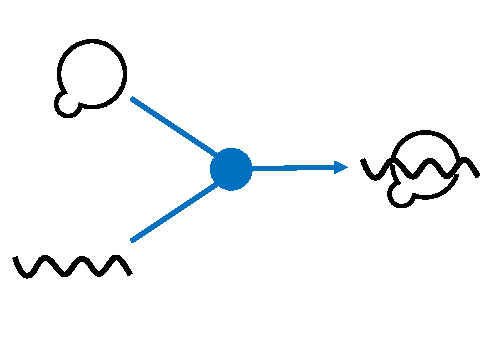
\includegraphics[scale=0.4]{figures/examples/4d-association.pdf}}
	\subfigure[MAY]{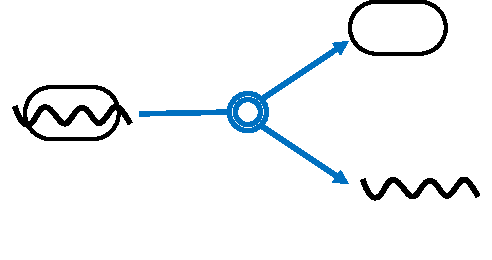
\includegraphics[scale=0.4]{figures/examples/4d-dissociation.pdf}}
	\subfigure[MAY]{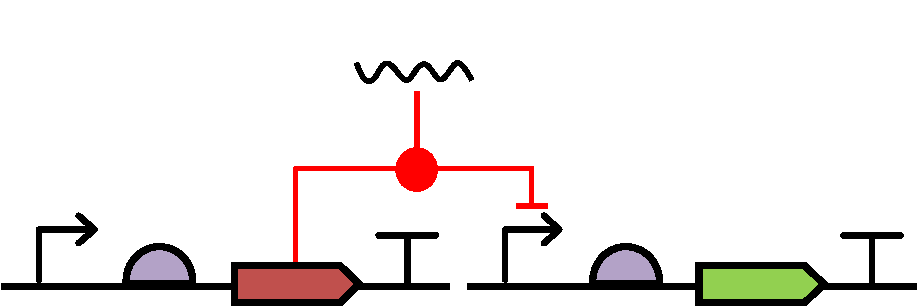
\includegraphics[scale=0.4]{figures/examples/4d-composite.pdf}}
	\subfigure[MUST NOT]{\includegraphics[scale=0.4]{figures/examples/4d-conflict.pdf}}
	\caption{Examples of use of multi-head and multi-tail arrows: 
	(a) Repression from multiple independent sources, (b) repressor with multiple targets, 
	(c) association of gRNA and Cas9 into an active CRISPR complex and (d) the dissociation of that complex, and
	(e) composite edges representing two interactions: CRISPR complex formation with dCas9 from two sources, which then represses a promoter.
	(f) Multi-head interactions, however, MUST NOT use different glyphs for different heads.}
	\label{exa:4d}
	\end{figure}

\item A biochemical process represented by a glyph at an edge junction SHOULD be represented using a glyph defined in \ref{apdx:sym:interactionnodes}. In this case, the interaction type MUST be contained within at least one of the glyph's associated terms.
In terms of the SBOL 2 data model, this means the glyph is equal to or a parent of at least one of the \sbol{types} for the \sbol{Interaction}, and that each associated \sbol{Participation} object has a \sbol{role} compatible with its position on the head or tail of the edge.
	Moreover, the glyph used SHOULD be the RECOMMENDED variant of the most specific applicable glyph.  Note that novel glyphs not defined in \ref{apdx:sym:interactionnodes} MAY be used, but SHOULD be proposed for adoption as described in \ref{sec:extension}.
}

\twotwozero{
	\begin{figure}[h!]
	\centering
	\subfigure[MAY]{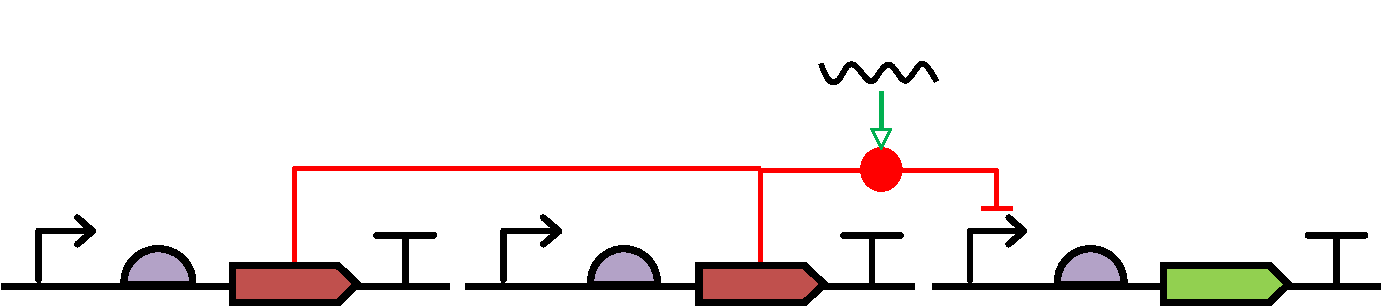
\includegraphics[scale=0.4]{figures/examples/4e-stimulate.pdf}}
	\subfigure[MAY]{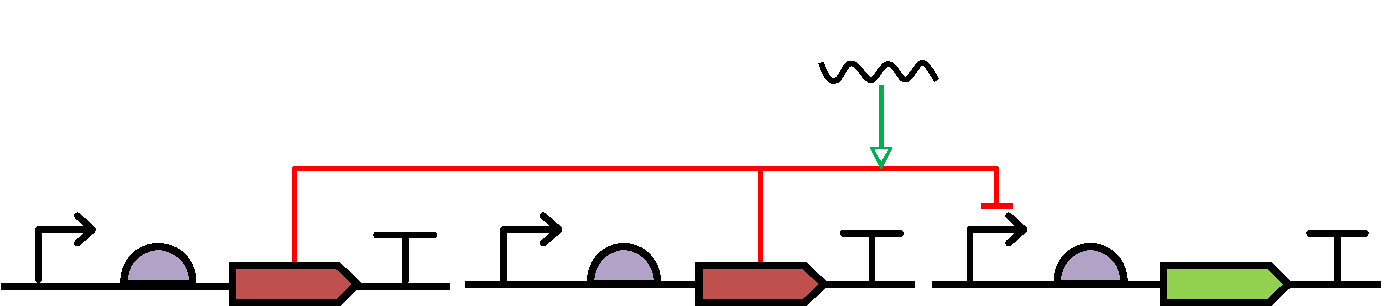
\includegraphics[scale=0.4]{figures/examples/4e-nodeless.pdf}}
	\subfigure[MUST NOT]{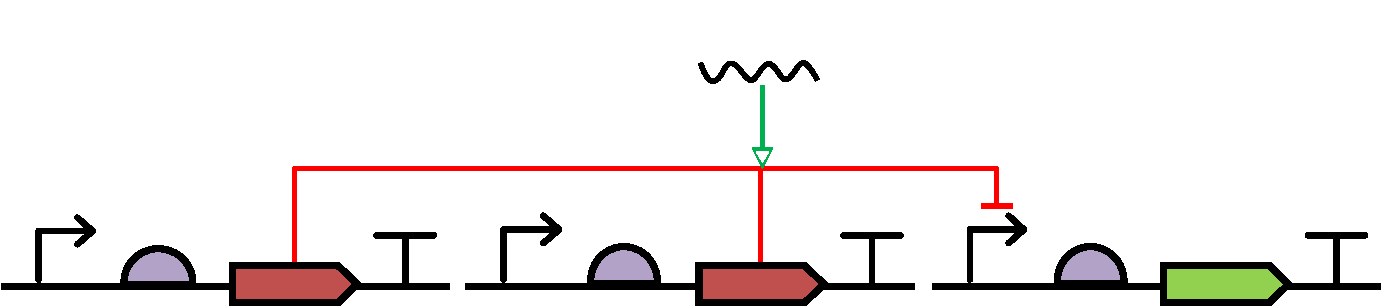
\includegraphics[scale=0.4]{figures/examples/4e-multiarrow.pdf}}
	\subfigure[MUST NOT]{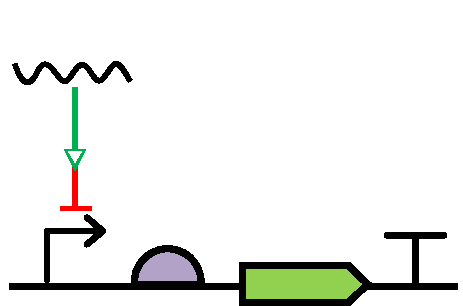
\includegraphics[scale=0.4]{figures/examples/4e-onearrow.pdf}}
	\caption{Examples of edges going into process nodes: 
	(a) gRNA stimulating the dCas9 repression process (an alternative Figure~\ref{exa:4d}(e) representation),  (b) the same but omitting the process node.
	The process node MUST NOT be omitted when there are more (c) or less (d) than one incoming and one outgoing edge.}
	\label{exa:4e}
	\end{figure}

\item An edge entering an edge junction may have an interaction arrow head (i.e., glyph from  \ref{apdx:sym:interaction}) to indicate the role its connected object plays in the biochemical process.
	If there is precisely one incoming edge without a head and precisely one outgoing edge, then the process node MAY be omitted, but otherwise MUST NOT be omitted.
	Examples are provided in~\ref{exa:4e}.
}

\end{enumerate}

\twoonezero{
\subsection{Modules}

A module within a system MAY be represented by a visual boundary in the form of closed polygon or closed curve.
Everything inside of the boundary is part of the module, and everything outside of the boundary is not part of the module; only certain diagram elements are allowed to cross a boundary, as defined below.
In terms of the SBOL 2 data model, the line represents a \sbol{Module} included within the \sbol{ModuleDefinition} represented by the surrounding diagram, and boundary-crossing elements define \sbol{MapsTo} relationships.
Note that the internals of a module need not be shown: some details can be omitted or a module can even be a ``black box'' with no internal structure at all being shown.

\begin{enumerate}
\item The boundary of module SHOULD should be a rectangle or rounded rectangle. Boundary sides SHOULD be oriented vertically and horizontally.  
	It is RECOMMENDED that a module be made visually distinct by making it larger than other glyphs and with a different line style.
	Examples are provided in~\ref{exa:moduleA}.

	\begin{figure}[h!]
	\centering
	\subfigure[SHOULD]{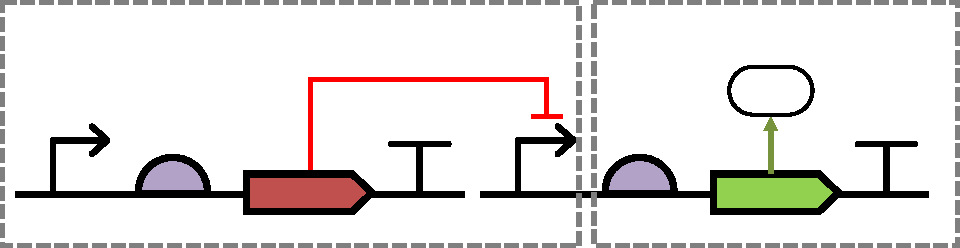
\includegraphics[scale=0.4]{figures/examples/moduleA-rectangle.pdf}}
	\subfigure[SHOULD]{\includegraphics[scale=0.4]{figures/examples/moduleA-roundrect.pdf}}
	\subfigure[SHOULD NOT]{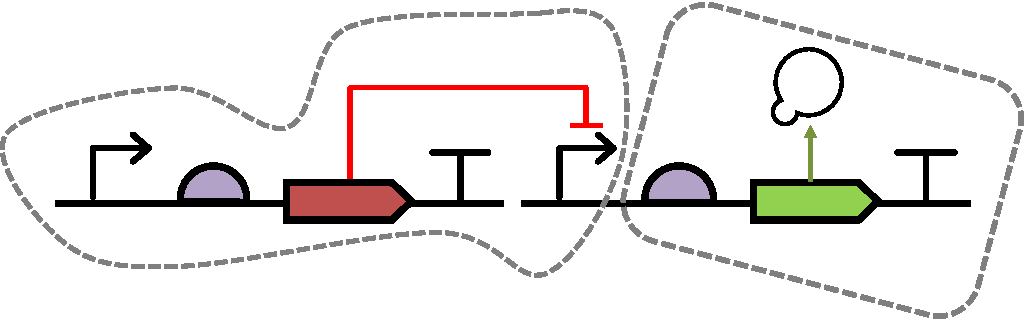
\includegraphics[scale=0.4]{figures/examples/moduleA-nonrect.pdf}}
	\subfigure[SHOULD NOT]{\includegraphics[scale=0.4]{figures/examples/moduleA-nondistinct.pdf}}
	\caption{Examples of recommended and problematic module boundaries: (a) two modules with visually distinct rectangular borders, (b) shows the same modules but with rounded rectangles and the second being a ``black box'' module with no internal structure shown, (c) shows modules with non-rectilinear borders, and (d) shows a black-box module that is not visually distinct from a sequence feature glyph.}
	\label{exa:moduleA}
	\end{figure}

\item An undirected edge (i.e., having no ``arrow head'') that crosses the boundary of a module represents a mapping associating the diagram elements that it links. 
Glyphs associated by a mapping MUST either be sequence features, molecular species, or module ports (see below), and must be of compatible types.
In terms of the SBOL 2 data model, the line represents a \sbol{MapsTo} relationship between a \sbol{FunctionalComponent} in the \sbol{ModuleDefinition} and another \sbol{FunctionalComponent} in the definition of the \sbol{Module}.
	Mapping edges SHOULD be made visually distinct from other lines in the same diagram, and it is RECOMMENDED that this distinction be made using dashed lines to represent mapping edges.
	Examples are provided in~\ref{exa:moduleB}.

	\begin{figure}[h!]
	\centering
	\subfigure[MAY]{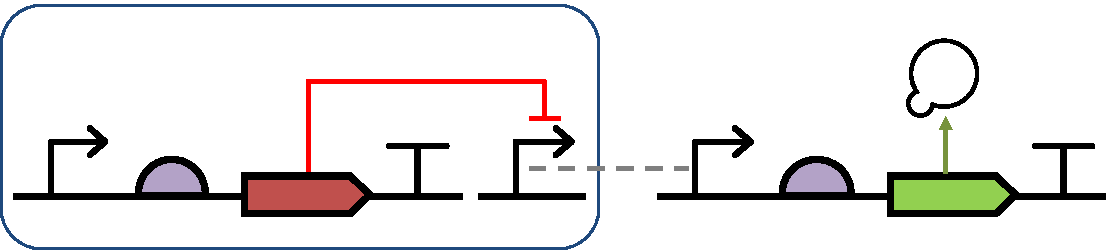
\includegraphics[scale=0.4]{figures/examples/moduleB-mapping.pdf}}
	\subfigure[SHOULD NOT]{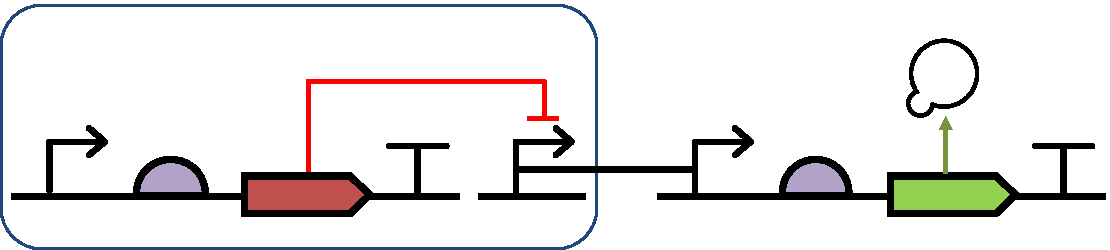
\includegraphics[scale=0.4]{figures/examples/moduleB-nondistinct.pdf}}
	\subfigure[MUST NOT]{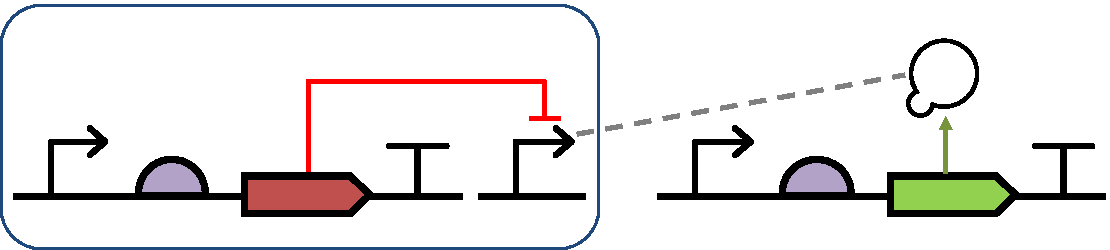
\includegraphics[scale=0.4]{figures/examples/moduleB-incompatible.pdf}}
	\caption{Examples of recommended and problematic mappings: (a) mapping showing that the promoter inside the module on the left is also used in the construct on the right, (b) mapping is not visually distinct from nucleic acid backbone, (c) mapping cannot identify a promoter with a macromolecule species.}
	\label{exa:moduleB}
	\end{figure}

\item Glyphs for sequence features and molecular species MUST NOT intersect with the boundary of a module.
	A nucleic acid backbone MAY cross the boundary of a module. This represents an implicit mapping between the region of the nucleic acid construct contained within the module and a compatible region of the larger construct represented in the enclosing system.
	An interaction edge MAY cross the boundary of a module. This represents an interaction in the enclosing system plus an implicit mapping between the component inside of the module and a compatible instance in the enclosing system.
	Examples are provided in~\ref{exa:moduleC}.

	\begin{figure}[h!]
	\centering
	\subfigure[MUST NOT]{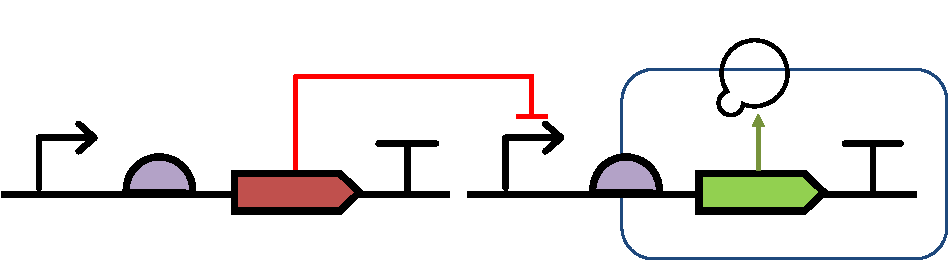
\includegraphics[scale=0.4]{figures/examples/moduleC-badcrossing.pdf}}\\
	\subfigure[MAY]{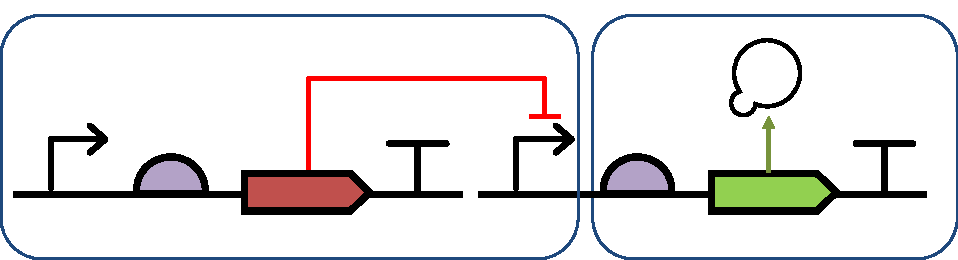
\includegraphics[scale=0.4]{figures/examples/moduleC-backbone.pdf}}
	\subfigure[MAY]{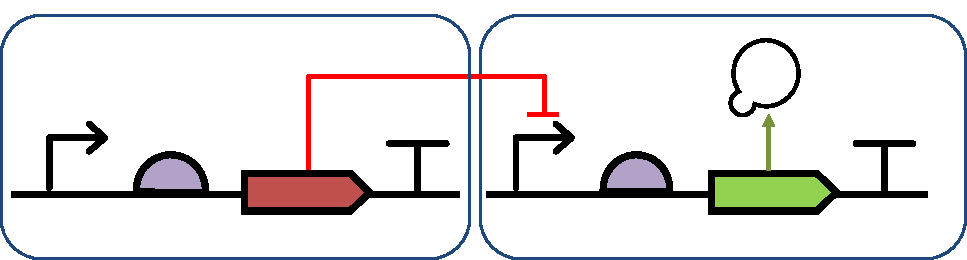
\includegraphics[scale=0.4]{figures/examples/moduleC-interaction.pdf}}
	\caption{Examples of recommended and problematic boundary intersections: (a) sequence feature and molecular species glyphs MUST NOT intersect a module boundary, (b) implicit mapping from the promoter in the left module and the regulated elements in the right module to a nucleic acid construct ordering both into a complete functional unit, (c) implicit mapping from the CDS in the left module and the promoter in the right module to instances in the complete system in which the CDS inhibits the promoter (presumably by a repressor product).}
	\label{exa:moduleC}
	\end{figure}


\item Small rectangles MAY be drawn on the outside of the module boundary to represent input/output ports.
In terms of the SBOL 2 data model, each rectangle is associated with a \sbol{FunctionalComponent} with a \sbol{direction} property that is \sbol{in}, \sbol{out}, or \sbol{inout}.
A port may be connected to an interaction edge head or tail to represent interactions with its associated component. 
%
If both a port and a glyph for its associated component are present in a diagram, then they MUST be visually connected, either explicitly by means of a mapping or implicitly by an interaction that passes through the port rectangle.
Likewise, mappings and interactions with the associated component MUST NOT cross the boundary except through the port.
%
A port SHOULD NOT both have interactions both connecting to it and crossing the boundary across it.
	Examples are provided in~\ref{exa:moduleD}.
% How do we show direction on a port?  We can't, really.

	\begin{figure}[h!]
	\centering
	\subfigure[MAY]{\includegraphics[scale=0.4]{figures/examples/moduleD-blackbox.pdf}}
	\subfigure[MAY]{\includegraphics[scale=0.4]{figures/examples/moduleD-mappings.pdf}}
	\subfigure[MAY]{\includegraphics[scale=0.4]{figures/examples/moduleD-interactions.pdf}}
	\subfigure[SHOULD NOT]{\includegraphics[scale=0.4]{figures/examples/moduleD-mixed.pdf}}
	\subfigure[MUST NOT]{\includegraphics[scale=0.4]{figures/examples/moduleD-disconnected.pdf}}
	\subfigure[MUST NOT]{\includegraphics[scale=0.4]{figures/examples/moduleD-evaded.pdf}}
	\caption{Examples of recommended and problematic module ports: (a) port on a black-box module, (b) ports connected to module internals via mappings, (c) boundary-crossing interaction passing through a port, (d) diagrams SHOULD NOT mix mappings and interactions on a give port, (e) ports MUST NOT be disconnected from their associated glyphs, and (f) if a port exists, interactions with that port MUST NOT cross the boundary at any other location.}
	\label{exa:moduleD}
	\end{figure}

\end{enumerate}
}

\subsection{Labels}
The name of any object in a diagram is RECOMMENDED to be displayed as text within, adjacent to, or otherwise clearly visually connected to the object's associated glyph.  In terms of the SBOL 2 data model, this is the \sbol{name} property, and if no \sbol{name} is supplied then the \sbol{displayId} MAY be used instead.
Examples are provided in~\ref{exa:5}.

	\begin{figure}[h!]
	\centering
	\includegraphics[width=3in]{figures/examples/5-labels.pdf}
	\caption{Examples of labels on glyphs.}
	\label{exa:5}
	\end{figure}


\subsection{Annotations}
Other text or graphics may be included as annotations with no constraint on their syntax or semantics.

\begin{enumerate}
\item Annotations SHOULD NOT be displayed in a way that allows them to be confused with other SBOL Visual elements.
\item Annotations SHOULD NOT be used to display information that can be displayed using other SBOL Visual elements.
\end{enumerate}

\subsection{Criteria for Compliance with SBOL Visual}

A diagram of a biological system is compliant with SBOL Visual if it complies with all MUST and MUST NOT requirements as specified above.
A diagram is compliant with SBOL Visual best practices if it also complies with all RECOMMENDED, SHOULD, and SHOULD NOT statements as specified above.

Importantly, note that a non-SBOL glyph can be used in a compliant
diagram when its definition is a subset or superset of a definition that
does have an SBOL Visual glyph.  For example, a diagram that creates a
new glyph for a special type of promoter can be SBOL Visual compliant
even though there is an SBOL Visual glyph for a general promoter.

A piece of software or other system for producing diagrams is
compliant with SBOL Visual under the following conditions:
\begin{enumerate}
\item The system MUST be capable of producing diagrams that are
  compliant with SBOL Visual.
\item If the system can also produce diagrams that are {\em not}
  compliant with SBOL Visual, it MUST clearly distinguish to the user
  between compliant and non-compliant usage and diagrams.
\end{enumerate}



\appendix
\appendixlabels

% -----------------------------------------------------------------------------
\section{SBOL Visual Glyphs}\label{apdx:symbols}
% -----------------------------------------------------------------------------

\todo[inline]{Check glyph specs for any SBOL 2 language}

The following pages present all current glyphs for SBOL Visual, organized by glyph families.
Each entry lists:
\begin{itemize}
\item Glyph family name
\item Associated ontology terms
\item Recommended and alternate glyphs
\item At least one example of when this glyph would be used
\item Any additional notes
\end{itemize}

\subsection{Sequence Feature Glyphs}\label{apdx:sym:feature}

These glyphs represent features of nucleic acid sequences, and include a bounding box (grey dashed box) and a recommended alignment to the nucleic acid backbone (grey dashed horizontal line).

% -----------------------------------------------------------------------------
\section{SBOL Glyphs}\label{sec:glyphs}
% -----------------------------------------------------------------------------

A glyph is a visual symbol used to represent an element in an SBOL Visual diagram.
All of the currently defined glyphs are collected in \ref{apdx:symbols}.
%
This section explains how glyphs are specified and how to add new glyphs.

Each SBOL glyph is defined by association with ontology terms, and can be used to represent any diagram element that is well-described by that term.
Currently there are four classes of glyphs, each associated with an ontology and a class in the SBOL 3 data model:
\begin{itemize}
\item {\bf Sequence Feature Glyphs} describe features of nucleic acid sequences. 
They are associated with Sequence Ontology terms.
For the SBOL 3 data model, this is formally defined as any \sbol{Feature} with a compatible term within its associated \sbol{roles},
 i.e., one that is equal to or a child of at least one term associated with the glyph.

\item {\bf Molecular Species Glyphs} represent any class of molecule whose detailed structure is not being shown using sequence feature glyphs. 
They are associated with Systems Biology Ontology terms. 
 For the SBOL 3 data model, this is formally defined as any \sbol{Feature} with a compatible term within its associated \sbol{types},
 i.e., one that is equal to or a child of at least one term associated with the glyph.

\item {\bf Interaction Glyphs} are ``arrows'' indicating functional relationships between sequence features, molecular species, and/or other relationships. 
They are associated with Systems Biology Ontology terms.
For the SBOL 3 data model, this is formally defined as any \sbol{Interaction} with a compatible term within its \sbol{types},
 i.e., one that is equal to or a child of at least one term associated with the glyph, 
 and with a compatible \sbol{Participation} at the head and tail of the arrow.

\item {\bf Interaction Node Glyphs} are placed at the junctions of edges to represent biochemical processes.
They are associated with Systems Biology Ontology terms.
For the SBOL 3 data model, this is formally defined as any \sbol{Interaction} with a compatible term within its \sbol{types},
 i.e., one that is equal to or a child of at least one term associated with the glyph, 
 and with a compatible \sbol{Participation} on the incoming and outgoing edges of the glyph
 \end{itemize}
 
More than one glyph may share the same definition: in this case, these glyphs form a family of variants, of which precisely one MUST be designated as the RECOMMENDED glyph, which is to be used unless there are strong reasons to prefer an alternative variant.

It will also frequently be the case that a diagram element could be represented by more than one glyph (e.g., a glyph for a specific term and a glyph for a more general term).
In such cases, it is RECOMMENDED that the most specific applicable glyph be used.
However, if upward branching in the relevant ontology means two applicable glyphs do not have an ordered parent/child relation, then either MAY be used.

For example, a protein coding sequence (CDS) is a sequence feature that may be represented either using the CDS glyph (Sequence Ontology term SO:0000316) or the Unspecified glyph (Sequence Ontology term SO:0000001).  
Since SO:0000316 is contained by SO:0000001, the preferred glyph is CDS, rather than Unspecified.
Likewise, a CDS may be represented by either a pentagonal glyph or an arrow glyph, but the pentagon is the RECOMMENDED variant, and so it is likewise preferred.  
\ref{f:glyphalternatives} illustrates this example.

\begin{figure}[h!]
\centering
\includegraphics[scale=0.6]{figures/glyphalternatives.pdf}
\caption{A biological design element such as a protein coding sequence (CDS) is best represented by the most specific RECOMMENDED glyph (middle), but can be represented by a less specific glyph such as Unspecified (left) or an approved alternative glyph (right).}
\label{f:glyphalternatives}
\end{figure}

Finally, note that the mapping from data model to glyph is not one-to-one: many SBOL 3 data model constructs can, at least in theory, be represented visually in multiple different ways. 
For example, a DNA construct carrying a heterologous gene could be represented by the molecular species glyph for a double-stranded nucleic acid, the sequence feature glyph for an engineered construct, or a series of sequence feature glyphs showing the internal structure of the gene.
This ambiguity is deliberate allowing diagrams to select an appropriate level of detail for the information that a diagram is intended to convey.

\subsection{Requirements for Glyphs}

\todo[inline]{Do we need to add to these for parametric?}

A number of requirements are placed on all SBOL Visual glyphs in order to
ensure both the clarity of diagrams and the ease with which they can
be constructed:
\begin{enumerate}
\item A glyph SHOULD have its meaning defined by associating the glyph with at least one ontology definition.
	Definitions are RECOMMENDED to be from the Sequence Ontology for sequence feature glyphs, from the Systems Biology Ontology for molecular species glyphs, and from the Systems Biology Ontology for interaction glyphs.  
	If no applicable terms are available in the preferred ontology, proposal of a new glyph SHOULD be accompanied by a request to the ontology maintainers to add a term for the undefined entity.  
\item A glyph SHOULD be relatively easy to sketch by hand (e.g., no high-complexity images or precise angles required).
\item A glyph specification MUST indicate which portions of the glyph are the ``interior'' for purposes of color fill.
\item A glyph specification SHOULD show the glyph in its preferred relative scale with respect to other glyphs.
\item A glyph SHOULD be specified using only solid black lines (leaving color and style to be determined by the user, as noted below).
\item A glyph SHOULD NOT be similar enough to be easily confused with any other glyph when written by hand, or when scaled either vertically, horizontally, or both.
\item A glyph SHOULD NOT include text (note that associated labels are not part of the glyph).
\end{enumerate}

In addition, some requirements apply only to certain classes of glyphs:
\begin{enumerate}[resume]
\item A sequence feature or molecular species glyph specification MUST include a rectangular bounding box indicating its extent in space.
\item A sequence feature glyph specification MUST include exactly one horizontal rule for its RECOMMENDED vertical alignment with the nucleic acid backbone.
\item A sequence feature glyph SHOULD be asymmetric on the horizontal axis. Vertical asymmetry is also preferred when possible.
\item If a sequence feature glyph can represent components of highly variable size or structural complexity, the glyph SHOULD be able to be scaled horizontally to indicate relative scale.
\end{enumerate}

\ref{f:specexample} shows examples of compliant glyph specification.

\begin{figure}[h!]
\centering
\includegraphics[scale=2.0]{figures/promoter-specification.pdf}
\includegraphics[scale=2.0]{figures/ribosome-entry-site-specification.pdf}
\caption{Examples of glyph specification: this specification for the sequence feature glyphs for Promoter (left) and Ribosome Entry Site (right) include the glyph outline, fill (grey center of Ribosome Entry Site), bounding box (dashed box), and recommended alignment with the nucleic acid backbone (dashed horizontal line), all at a preferred relative scale.}
\label{f:specexample}
\end{figure}

\subsection{Reserved Visual Properties}

SBOL Visual aims to allow as much flexibility and freedom as possible in how diagrams are organized, presented, and styled.
%
To this end, a number of aspects of presentation are generally reserved for the communication of other types of information by the creator of a diagram.
%
When using a glyph in a diagram, the following choices in glyph presentation are thus explicitly intended to be alterable:
\todo[inline]{Do we need to add to these for parametric?}
\begin{enumerate}
\item The lines of a glyph MAY be given any line thickness and style
\item The interior of a glyph MAY be given any fill color, as long as the choice of fill does not interfere with recognizing the glyph.
\item The scale of glyphs are RECOMMENDED to be kept consistent with their specification and throughout a diagram, but can be altered if desired, particularly to convey additional information (e.g., length of a sequence).
\item Minor styling effects MAY be chosen (e.g., shadow, corner styling, other "font-level" customization)
\end{enumerate}
\ref{f:stylevariation} shows some examples of acceptable style variation.

In certain special cases, the style of a glyph may be more constrained, but such cases are expected to be rare and strongly motivated.

\begin{figure}[h!]
\centering
\includegraphics[scale=1.0]{figures/style-variation.pdf}
\caption{Examples of acceptable style variation for a Promoter glyph.}
\label{f:stylevariation}
\end{figure}

\subsection{Extending the Set of Glyphs}\label{sec:extension}
The collection of SBOL Visual glyphs is not expected to provide
complete coverage of all of the types of element that people will
wish to include in genetic diagrams, particularly given the ongoing
evolution of synthetic biology as an engineering discipline.
%
As the need for new diagram elements or new practices of usage emerge,
new glyphs or glyph definitions are expected to be added to SBOL
Visual.
%
In particular, the following three classes of changes are expected to occur regularly,
and the SBOL development community will maintain clear processes for
proposal and adoption of changes of this type:
\begin{itemize}
\item New glyphs, either representing a type of component that
  previously lacked a glyph or enabling a distinction between types of
  components previously represented by the same glyph.
\item Additional glyph variants, accompanied by compelling use cases
  that cannot be adequately addressed by the existing glyph variants.
\item Additional definitions for a glyph, capturing an alternate
  meaning that is useful to humans but existing within a disjoint
  branch of the relevant ontology.
\end{itemize}

In order to support the coherent extension of SBOL Visual, 
whenever a diagram creator uses a glyph not found in \ref{apdx:symbols}, 
the creator SHOULD submit it to be considered for inclusion in an updated version of the standard following the processes for adding new glyphs found on the community website at \url{http://sbolstandard.org}






\subsection{Molecular Species Glyphs}\label{apdx:sym:species}

These glyphs represent molecular species in a diagram, and include a bounding box (grey dashed box) but are not connected to any nucleic acid backbone.

% Autogenerated glyph page collection, do not edit by hand
\twothreezeronopage{
\includepdf[pagecommand={},pages={1-}]{glyphscript/Glyphs/FunctionalComponents/complex.pdf}
}
\twotwozeronopage{
\includepdf[pagecommand={},pages={1-}]{glyphscript/Glyphs/FunctionalComponents/dsNA.pdf}
}
\twotwozeronopage{
\includepdf[pagecommand={},pages={1-}]{glyphscript/Glyphs/FunctionalComponents/macromolecule.pdf}
}
\twotwozeronopage{
\includepdf[pagecommand={},pages={1-}]{glyphscript/Glyphs/FunctionalComponents/no-glyph-assigned.pdf}
}
\twotwozeronopage{
\includepdf[pagecommand={},pages={1-}]{glyphscript/Glyphs/FunctionalComponents/protein.pdf}
}
\twotwozeronopage{
\includepdf[pagecommand={},pages={1-}]{glyphscript/Glyphs/FunctionalComponents/simple-chemical.pdf}
}
\twotwozeronopage{
\includepdf[pagecommand={},pages={1-}]{glyphscript/Glyphs/FunctionalComponents/ssNA.pdf}
}
\twotwozeronopage{
\includepdf[pagecommand={},pages={1-}]{glyphscript/Glyphs/FunctionalComponents/unspecified.pdf}
}



\subsection{Interaction Glyphs}\label{apdx:sym:interaction}

These glyphs are different forms of ``arrow'' representing interactions between sequence features and/or molecular species. As arrows, they are extensible and do not have a separately identified bounding box.

% Autogenerated glyph page collection, do not edit by hand
\includepdf[pagecommand={},pages={1-}]{glyphscript/Glyphs/Interactions/control.pdf}
\includepdf[pagecommand={},pages={1-}]{glyphscript/Glyphs/Interactions/degradation.pdf}
\includepdf[pagecommand={},pages={1-}]{glyphscript/Glyphs/Interactions/inhibition.pdf}
\includepdf[pagecommand={},pages={1-}]{glyphscript/Glyphs/Interactions/process.pdf}
\includepdf[pagecommand={},pages={1-}]{glyphscript/Glyphs/Interactions/stimulation.pdf}


\twoonezero{
\subsection{Interaction Node Glyphs}\label{apdx:sym:interactionnodes}

These glyphs are placed at the junctions of edges to represent biochemical processes, and include a bounding box (grey dashed box) but are not connected to any nucleic acid backbone. Grey dashed lines provide examples of how edges may connect to the glyph.
}

% Autogenerated glyph page collection, do not edit by hand
\includepdf[pagecommand={},pages={1-}]{glyphscript/Glyphs/InteractionNodes/association.pdf}
\includepdf[pagecommand={},pages={1-}]{glyphscript/Glyphs/InteractionNodes/dissociation.pdf}
\includepdf[pagecommand={},pages={1-}]{glyphscript/Glyphs/InteractionNodes/process.pdf}
\includepdf[pagecommand={},pages={1-}]{glyphscript/Glyphs/InteractionNodes/unspecified.pdf}



% -----------------------------------------------------------------------------
\section{Examples}\label{sec:examples}
% -----------------------------------------------------------------------------

This section contains prototypical examples, including use of all
current glyphs to attempt to ensure that their use is clear.

\begin{figure}[h!]
\includegraphics[scale=0.5]{figures/apdx-examples/apdx-exa1.pdf}
\caption{DNA sequence for a functional unit in which the pTet promoter and an anonymous ribosome entry site regulate expression of a coding sequence for GFP, ended by a terminator.}
\label{f:apdx:exa1}
\end{figure}

\begin{figure}[h!]
\includegraphics[scale=0.5]{figures/apdx-examples/apdx-exa2.pdf}
\caption{The same functional unit as in \ref{f:apdx:exa1}, with additional assembly-focused information: there is a 5' overhang before the promoter, a 3' overhand after the terminator, and an assembly scar between the promoter and the ribosome entry site left over from a prior step of assembly.}
\label{f:apdx:exa2}
\end{figure}

\begin{figure}[h!]
\includegraphics[scale=0.5]{figures/apdx-examples/apdx-exa3.pdf}
\caption{Promoter pTet stored in a circular plasmid. The promoter is prepared for being cut out of the plasmid: it is preceded by a 5' sticky end restriction site and followed by a 3' stick end restriction site.  In addition, the plasmid has been bar-coded with a signature and has its origin of replication marked.}
\label{f:apdx:exa3}
\end{figure}

\begin{figure}[h!]
\includegraphics[scale=0.5]{figures/apdx-examples/apdx-exa4.pdf}
\caption{Promoter stored in a plasmid as in \ref{f:apdx:exa3}, except that the restriction sites before and after the promoter are blunt-end.}
\label{f:apdx:exa4}
\end{figure}

\begin{figure}[h!]
\includegraphics[scale=0.5]{figures/apdx-examples/apdx-exa5.pdf}
\caption{Promoter stored in a plasmid as in \ref{f:apdx:exa3}, except that the cut structure of the restriction sites before and after the promoter is not specified.}
\label{f:apdx:exa5}
\end{figure}

\begin{figure}[h!]
\includegraphics[scale=0.5]{figures/apdx-examples/apdx-exa6.pdf}
\caption{Promoter stored in a plasmid as in \ref{f:apdx:exa3}, except that there is a ribonuclease site after the promoter rather than restriction sites flanking it.}
\label{f:apdx:exa6}
\end{figure}

\begin{figure}[h!]
\includegraphics[scale=0.5]{figures/apdx-examples/apdx-exa7.pdf}
\caption{Detailed design of a promoter, in which the transcription start site is preceded by two operator sites where regulators bind, and the whole is flanked by insulators.}
\label{f:apdx:exa7}
\end{figure}

\begin{figure}[h!]
\includegraphics[scale=0.5]{figures/apdx-examples/apdx-exa8.pdf}
\caption{Promoter regulating the production of an engineered composite sequence that includes RNA and protein stability elements at its 3' end, as well as an internal site for protease cleavage, as well as the expansion of the composite to show it contains a ribosome entry site. coding sequence, and other omitted details.  Single residue locations of interest are indicated for the DNA (before the promoter), RNA (after the ribosome entry site), and protein (in the CDS).}
\label{f:apdx:exa8}
\end{figure}

\begin{figure}[h!]
\includegraphics[scale=0.5]{figures/apdx-examples/apdx-exa9.pdf}
\caption{DNA sequence with three primer binding sites.}
\label{f:apdx:exa9}
\end{figure}

\begin{figure}[h!]
\includegraphics[scale=0.5]{figures/apdx-examples/apdx-exa10.pdf}
\caption{The same functional unit as in \ref{f:apdx:exa1}, except that information about the CDS is missing, leaving it to fall back on the default unspecified glyph.}
\label{f:apdx:exa10}
\end{figure}

\twothreezero{
\begin{figure}[h!]
\includegraphics[scale=0.5]{figures/apdx-examples/apdx-exa11.pdf}
\caption{Promoter regulating the expression of GFP, which is also regulated by an aptamer between it and the poly-A tail of the transcript. The promoter can be cut out by a pair of recombinase target sites, which are acted on by the Flp protein.  The whole construct is stored in a circular plasmid with an origin of replication and also an origin of transfer.}
\label{f:apdx:exa11}
\end{figure}
}

\begin{figure}[h!]
\includegraphics[scale=0.5]{figures/apdx-examples/apdx-exa12.pdf}
\caption{Promoter stimulated by the CDS that it regulates.}
\label{f:apdx:exa12}
\end{figure}

\twothreezero{
\begin{figure}[h!]
\includegraphics[scale=0.5]{figures/apdx-examples/apdx-exa13.pdf}
\caption{Constitutive production of TetR, except that information about the protein is missing, leaving it as the default unspecified glyph. TetR represses the pTet promoter, which is regulating production of GFP.  The diagram of GFP production explicitly includes the intermediate mRNA and the degradation of both the mRNA and protein products.}
\label{f:apdx:exa13}
\end{figure}

\begin{figure}[h!]
\includegraphics[scale=0.5]{figures/apdx-examples/apdx-exa14.pdf}
\caption{Phosphorylation of an inactive transcription factor (produced by two different CDSs) by a kinase to form an active transcriptional activator, which then stimulates a promoter.}
\label{f:apdx:exa14}
\end{figure}

\begin{figure}[h!]
\includegraphics[scale=0.5]{figures/apdx-examples/apdx-exa15.pdf}
\caption{Ribozyme and spacer between two transcriptional units, forming a separation module with the preceding terminator (dashed box), with the whole construct integrated into the chromosome.}
\label{f:apdx:exa15}
\end{figure}

\begin{figure}[h!]
\includegraphics[scale=1.0]{figures/apdx-examples/apdx-exa16-circular-plasmid-example.pdf}
\caption{A circular plasmid containing a functional unit consisting of promoter, ribosome entry site, CDS, and terminator.}\label{f:apdx:exa16}
\end{figure}

\begin{figure}[h!]
\includegraphics[scale=1.0]{figures/apdx-examples/apdx-exa17-chromosomal-locus-example.pdf}
\caption{A functional unit consisting of promoter, ribosome entry site, CDS, and terminator, all integrated together into the chromosome.}
\label{f:apdx:exa17}
\end{figure}

\begin{figure}[h!]
\includegraphics[scale=1.0]{figures/apdx-examples/apdx-exa18-chromosomal-locus-example2.pdf}
\caption{Two functional units, one integrated into the amyE locus, another integrated into the ganA locus}\label{f:apdx:exa18}
\end{figure}

\begin{figure}[h!]
\includegraphics[scale=0.5]{figures/apdx-examples/apdx-exa19-stop-sites.pdf}
\caption{Coding sequence marking the stop codon at its end and transcriptional end site farther down the sequence.}
\label{f:apdx:exa19}
\end{figure}

\begin{figure}[h!]
\includegraphics[scale=1.0]{figures/apdx-examples/apdx-exa20-intron.pdf}
\caption{A coding sequence with three domains: an N-tag (blue), C-tag (yellow), and internal region (red) interrupted by an intron that includes a gRNA non-coding RNA sequence (green).}
\label{f:apdx:exa20}
\end{figure}

\begin{figure}[h!]
\includegraphics[scale=1.0]{figures/apdx-examples/apdx-exa21-polypeptide-region.pdf}
\caption{A coding sequence with three designated domains, an N-tag (blue), C-tag (yellow), and internal region (red).}
\label{f:apdx:exa21}
\end{figure}

\begin{figure}[h!]
\includegraphics[scale=0.75]{figures/apdx-examples/apdx-exa22.pdf}
\caption{The AraC protein and arabinose associating into a complex that activates the pBAD promoter.}
\label{f:apdx:exa22}
\end{figure}

\begin{figure}[h!]
\includegraphics[scale=0.75]{figures/apdx-examples/apdx-exa23-bicistronic.pdf}
\caption{Bicistronic expression of both GFP and RFP from a signal coding sequence, by means of a 2A self-cleaving polypeptide region.}
\label{f:apdx:exa23}
\end{figure}


}

% Figure black magic: adjust the size here as needed to get the spacing on the last page of the section correct.
%\begin{figure}[h!]
%\vspace{2in}
%\end{figure}




% -----------------------------------------------------------------------------
\section{Relationship to SBOL Visual 1.0}\label{sec:sbol1}
% -----------------------------------------------------------------------------

SBOL Visual 2.0 differs from SBOL Visual 1.0 in the following major ways:
\begin{itemize}
\item Diagram syntax is expanded to include functional interactions and other molecular species.
\item The relationship between diagrams and the SBOL data model is made explicit.
\item A number of requirements and best practices are specified for glyphs and diagrams, including:
	\begin{itemize}
	\item Glyphs include information on interior, bounding box, and recommended backbone alignment.
	\item Sequence feature glyphs are required to have their bounding boxes contact the nucleic acid backbone.
	\item Nucleic acid diagrams now require the nucleic acid backbone line, and the number of lines allowed in various circumstances is constrained.
	\item Explicit statement of when a glyph can and cannot be used to represent a particular element of a diagram.
	\end{itemize}
\item Labels that name objects are distinguished from other types of textual annotation.
\item Explicit statement of which aspects of a symbol are {\em not} controlled.
\item Symbol variants are now supported.
\end{itemize}

In addition, the collection of sequence feature glyphs have been expanded and modified in the following ways:
\begin{itemize}
\item All non-ambiguous glyphs have been provided with bounding box, interior, and recommended backbone alignment.
\item The User Defined glyph has been split into Unspecified, No Glyph Assigned, Engineered Region, and Composite. 
\item Glyphs have been added for Aptamer, Omitted Detail, Biopolymer Location, Non-Coding RNA Gene, Origin of Transfer, PolyA Site, and Specific Recombination Site.
\item The following ontology terms have been assigned or adjusted: 
	\begin{itemize}
	\item Ribonuclease Site has been assigned SO:0001977.
	\item 5' Sticky End Restriction Site has been assigned SO:0001975.
	\item 3' Sticky End Restriction Site has been assigned SO:0001976.
	\item Signature has been assigned SO:0001978.
	\item RNA Stability Element has been updated from the obsolete SO:0001957 to the current SO:0001979
	\item Restriction Enzyme Recognition Site, in addition to SO:0000139 has a second definition as SO:0000061.
	\item 5' Overhang Site and 3' Overhang Site were erroneously listed with their ontology terms exchanged; this has been fixed.
	\end{itemize}
\end{itemize}


\newpage
\label{s:bibliography}
\bibliography{sbol}

\end{document}
